\documentclass[a4paper,12pt]{kth-mag}
\usepackage[T1]{fontenc}
\usepackage{textcomp}
\usepackage{lmodern}
\usepackage[utf8x]{inputenc}
\usepackage[swedish,english]{babel}
\usepackage{modifications}
\usepackage{minted}
\usepackage{cite}
\usepackage{graphicx}
%\usepackage{float}
% IMPORTANT! This need to be the last package loaded since it overwrites features from others to work correctly
\usepackage[pdfusetitle=true, pdfauthor={Pascal Chatterjee and Joakim Carselind}, pdfsubject={Bachelors essay 2012 (dkand12) in computer science and communication at Royal Institute of Technology, Stockholm, Sweden}, pdfkeywords={Concurreny,JVM,Java,Groovy,Clojure}, pdftex]{hyperref}

\definecolor{code}{rgb}{0.95,0.95,0.95}
\raggedbottom % force text to top

\title{Concurrency on the JVM}

\subtitle{An investigation of strategies for handling concurrency in Java, Clojure and Groovy}
          
\foreigntitle{En undersökning av strategier för hantering av parallellism i Java, Clojure och Groovy}
              
\author{Pascal Chatterjee \and Joakim Carselind \\ \small{\{pascalc, joacar\}@kth.se}}
\date{April 2012}

\blurb{Bachelor's Thesis at NADA\\Supervisor: Mads Dam\\Examiner: Mårten Björkman}
\trita{TRITA xxx 2012-nn}

% Magic
\makeatletter\@addtoreset{section}{part}\makeatother%
\renewcommand{\thesection}{\arabic{section}}

\begin{document}

\frontmatter
\pagestyle{empty}
\removepagenumbers
\maketitle
\selectlanguage{english}

\begin{abstract}
    Processors with multiple cores opens up for better utilisation of hardware resources for applications if they take advantage of concurrency and parallelism. There are several methods to reap the benefits of concurrency; software transactional memory, actors and agents, locks and threads. The use of parallelism in programming comes at a price: synchronisation between threads operating on shared memory resources.

New software libraries and programming language exists to simplify implementation of parallel application and this essay investigate strategies on those with the Java Virtual Machine as a commonon denominator: Java, Clojure and Groovy.
\endinput
\end{abstract}

\clearpage

\begin{foreignabstract}{swedish}
  Flerkärniga processorer skapar grund för bättre nyttjande av hårdvaruresurser för applikationer implementerade parallelt. Det existerar ett flertal methoder för att skörda fördelarna av parallelism: software transactional memory, skådespelare och agenter, lås och trådar. Men parallelism har ett pris: att synkronisera trådarna som arbetar på delade minnesresurser.

Nya mjukvarubibliotek och programeringsspråk existerar för att förenkla implementationen av parallella applikationer och i denna uppsats undersöker vi de som har en gemensam nämnare Javas virtuella maskin: Java, Clojure och Grooy. 
\endinput
\end{foreignabstract}

\clearpage

\tableofcontents*
\mainmatter
\pagestyle{newchap}
\makeatletter\@openrightfalse

\chapter{Introduction}

\section{Statement of collaboration}
The code included in appendix and elsewhere is a product of Pascal Chatterjee and figures are a product of Joakim Carselind. The text is a collaborative outcome of our findings performing the practical investigation and deepening our knowledge by reading papers, articles and books in the subject of concurrency and related subjects.

\section{Delimiation of study}
To limit the area of study, we will investigate concurrency in the context of a bank transfer situation, where a withdrawal is followed by a deposit. The system contains a predefined amount and the correctness of the system is tested by issuing several \texttt{withdraw} and \texttt{deposit} operations in parallel and observering the amount of money after these operations have been performed.

With this said, the result should not be viewed as the best language to use to create a large system as we will not have time to set up a large system and perform extensive test taking robustness, safety, availability and performance into consideration.

\section{Problem statement}
To reach better utilisation of hardware resources, an increasing key factor for companies providing IT solutions in order to be competetive and profitable, one must leverage the full potential of multi-core processors. The rapid development of distributed computing and concurrent applications require robust and scalable software architecture to reap the benefits from concurrency.

To design concurrent applications is complicated but how could one make it less complicated to implement?

\section{Introduction}
More cores let the computer execute instructions like add or move parallel which could increase the performance of a software application. However, the potential performance gain comes with a price namely increased control over synchronisation to prevent memory corruption in shared memory resources. Since traditional sequential execution is, to some extent, abandoned for concurrent execution, a situation arise that could cause the application to behave non-deterministically.

For this reason, synchronisation plays a crucial role to maintain consistency and correctness in concurrent environments.

Applications that consists of mutually exclusive operations such as distributed database queries performs well under concurrency whilst applications tackling a computationally hard problem might see no or insignificant performance gain when implemented with a parallel design.

Modern, dynamic languages like Ruby and Python feature a \textit{Global Interpreter Lock} (GIL), so we need to use languages such as C/C++/Java to leverage multiple processors. We will focus on the JVM in this paper.  

\part{Introducing concurrency}

\section{Concurrency control} \label{sec:con_con}
Concurrency control defines guidelines to maintain data integrity and achieve correctness in concurrent environments such as hardware modules and operating systems\cite{concon}. When modules, regarding level, communicate concurrently there is a risk of the data integrity being violated. The consequence could be that the system stop working or, even worse, continue without any outer signs of an error occured. If situations like this occurs, they may be extremely difficult to reproduce and debug. Therefore the use of concurrency control is highly important to make sure that the system conforms to rules applicable for concurrent environments.

\section{Threads and processes}
A process is generally created and managed by the operating system and have its own state, address space and communicates using an interprocess protocol.

Threads, as opposed to processes, share state, address space and communicate directly since they share address space and hence variables. Threads are spawned by a process and typically suited to perform tasks not requiring a linear solving approach, i.e. the task could be parallelised. When a thread has completed its task, it is absorbed by the process that created it.

The existence of multiple threads inside a process brings up a risk of different threads operating on the same memory resource and due to this synchronisation is important to maintain correctness. The operations performed by threads need to be \textbf{atomic} if they execute code in a \textbf{critical section} in the context of the process memory and shared mutuable resources.

\section{Atomicity}

One of the first things we should realise when writing concurrent programs is that most of the statements we use are \textit{not} \textbf{atomic}. This means that although we tend to think of them as indivisible units of computation, they expand to multiple instructions when compiled to bytecode. It is these instructions that are atomic, not the statements we write in high-level languages.

Let us take the simple example of incrementing an integer variable. In Java, we could write the function:

\begin{listing}[H]
\begin{minted}[linenos=true,bgcolor=code]{java}
public static void add(int var, int num) { 
	var = var + num; 
}
\end{minted}
\end{listing}

Intuitively, we might think that that if a context switch were to occur in our function, it would take place at line 1, 2 or 3. This would be the case if line 2 was atomic, but as it consists of addition \textit{and} assignment, it is compiled to multiple bytecode instructions. We can see these instructions here:

\begin{listing}[H]
	\begin{minted}[linenos=true,bgcolor=code]{java}
public static void add(int, int);
	iload_0
	iload_1
	iadd
	istore_0
	return
  	\end{minted}
\end{listing}

The second line from our Java \texttt{add} function generates the \texttt{iadd} and \texttt{istore0} instructions at lines 4 and 5 of the bytecode. 

It is entirely possible for a thread switch to occur in between these instructions. Usually this is not problematic at all, and in fact this happens many times a second on all modern operating systems. However, if multiple threads attempt to change the value of the \textit{same} variable at the same time, inconsistencies begin to arise. 

\section{Shared memory}

In order to better illustrate the lack of atomicity in our add function, we can rewrite it to look like this:

\begin{listing}[H]
	\begin{minted}[linenos=true,bgcolor=code]{java}
public static void add(int num) 
throws InterruptedException {
        int v = var;
        Thread.sleep(1);
        var = v + num;
}
  	\end{minted}
\end{listing}

Here \texttt{var} is an instance variable. The \texttt{Thread.sleep} at line 4 forces a context switch after \texttt{var} has been copied to the local variable \texttt{v}. If any other thread alters \texttt{var} during this time, those changes will be lost when the original thread resumes and writes \texttt{v + num} back to \texttt{var}. The following could well happen if two threads were to execute \texttt{add} simultaneously:

\begin{listing}[H]
	\begin{minted}[linenos=true,bgcolor=code]{java}
   // var = 0
   // Thread 1
    int v = var; // v = 0
    Thread.sleep(1);
    // * Context Switch *
        // Thread 2
        int v = var // v = 0
        Thread.sleep(1)
        var = v + 1 // var = 1
        // * Context Switch *
    var = v + 1; // var = 1
  	\end{minted}
\end{listing}

As we can see, after this interleaving of statements, \texttt{var = 1} even though it was incremented \textit{twice}. It is in this way that shared mutable memory, or state, can lead to inconsistent data even though the program logic is correct. We call this phenomenon - when the result of a program is dependent on the sequence or timing of other events - a \textbf{race condition}.

\begin{figure}[H]
\begin{center}
    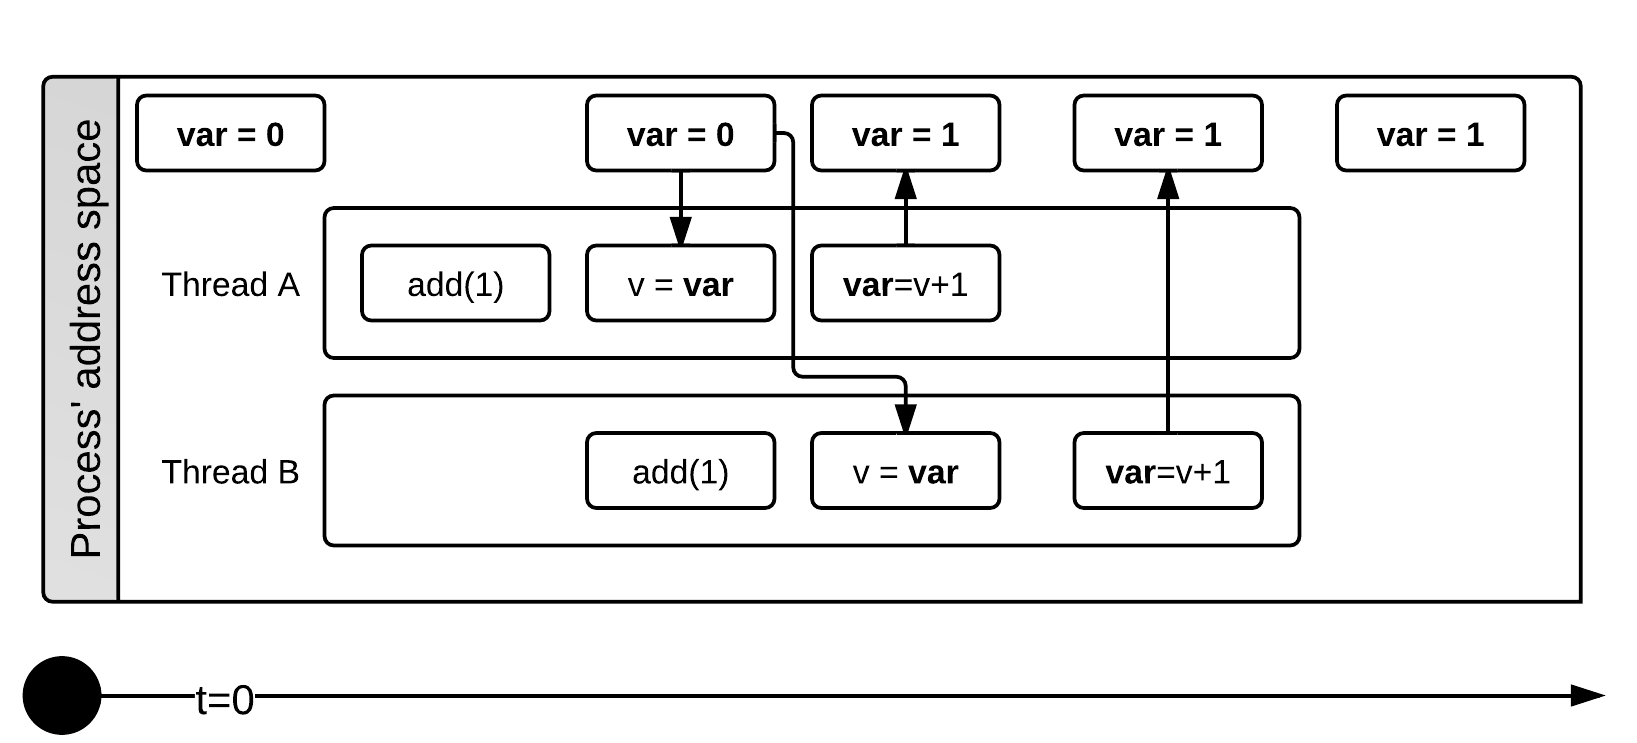
\includegraphics{images/ProcessAndThreads.png}
\caption{Process and threads synchronisation issue.}\label{fig:pat_sync_issue}
\end{center}
\end{figure}

All of the concurrency strategies discussed in this paper aim to mitigate the effects of race conditions, and thereby ensure that programs behave in a deterministic way despite the activity of multiple threads. They do this by eliminating one of the factors from \textbf{uncontrolled access to shared, mutable state} that can lead to problems. The first approach we consider, threads and locks, uses locks to \textbf{control access} to shared mutable state.

\part{Threads and Locks}

\section{Background}
When an application is initiated from the operating system, a process is created to host the application and it is allocated working primary memory (random access memory). Typically there are many processes running simultaneously and each process can spawn multiple threads. Since threads share the address space, they share variables which implies a risk of executing overlapping operations on the same resource and synchronisation of resources is crucial.

A bank account that allow withdrawals, deposits and reading the value of a balance is used to illustrate the concurrency strategies in this paper. Formally this could be viewed as an interface, that in Java can be written:

\begin{listing}[H]
	\begin{minted}[linenos=true,bgcolor=code]{java}
public interface Account {
    public float getBalance();
    public boolean deposit(float amount);
    public boolean withdraw(float amount);
}
  	\end{minted}
\end{listing}

\texttt{getBalance} returns the current balance as a \texttt{float}; \texttt{deposit} and \texttt{withdraw} increment and decrement the current balance respectively, and return a boolean signifying whether they succeeded. \texttt{withdraw} can fail if more funds are requested than are present in the balance.

\newpage

\section{No locks}

We begin by implementing the \texttt{Account} interface in the simplest possible way.

\begin{listing}[H]
	\begin{minted}[linenos=true,bgcolor=code]{java}
public class NaiveAccount implements Account {
    private float balance = 0;

    public float getBalance() {
    		Thread.sleep(1);
        return balance;
    }

    public void deposit(float amount) 
    throws InterruptedException {
        float b = balance;
        Thread.sleep(1);
        balance = b + amount;
    }

    public void withdraw(float amount) 
    throws InterruptedException {
        float b = balance;
        Thread.sleep(1);
        balance = b - amount;
    }
}  
	\end{minted}
\end{listing}

As we explained in section 1.3, we insert a \texttt{Thread.sleep} in the middle of \texttt{deposit} and \texttt{withdraw} in order to highlight the danger of context switches.

\subsection{Testing correctness}

We can (informally) test the correctness of this implementation by initially depositing a certain amount in an account, carrying out a certain number of deposits and withdrawals, and then making sure that the resulting balance is as we expected.

In these tests the initial balance is \texttt{10}, and we carry out a sequence of 10 deposits and 10 withdrawals, each for the amount of \texttt{1} unit. As these cancel out, our finishing balance should also be \texttt{10} as that is what we started with. These operations are themselves carried out 10 times to see what happens when they are repeated.

\subsubsection{Single Threaded}

The collected final balances of the single threaded tests are shown below:

\begin{listing}[H]
	\begin{minted}[bgcolor=code]{java}
[10.0, 10.0, 10.0, 10.0, 10.0, 10.0, 10.0, 10.0, 10.0, 10.0]
	\end{minted}
\end{listing}

As we can see, these final balances are exactly what we would expect given an initial balance of 10, followed by 10 deposits and 10 withdrawals of 1 unit. The results were also unchanged over the course of 10 trials.

\subsubsection{Multiple Threaded}

Now let's see what happens when we run the withdrawals and the deposits in separate threads. 

\begin{listing}[H]
	\begin{minted}[bgcolor=code]{java}
[8.0, 20.0, 20.0, 20.0, 6.0, 0.0, 16.0, 18.0, 8.0, 0.0]
	\end{minted}
\end{listing}

Here the final balance ranged between 0 and 20, which is an error of $-10 \leq error \leq 10$. This shows that in some runs all our withdrawals disappeared; in others all our deposits disappeared; and sometimes we saw a mixture of these two extremes. Such disappearances of actions from our results happened when a certain interleaving of statements from the two threads occurred as described in section 1.3.

\begin{table}[h]
    \centering
    \begin{tabular}{| l | c |} 
    \hline
    \textbf{Mean} & \$11.6 \\
    \textbf{Deviation} & \$7.2 \\
    \hline 
    \end{tabular}
    \caption{1 000 runs of non-thread safe bank transfer application shows a highly non-deterministic behaviour.}
\end{table}

This makes it very obvious that the \texttt{deposit} and \texttt{withdraw} methods are \textbf{critical sections} - a section of code that should only be executed by one thread at any time. These sections need to be \textbf{mutually exclusive} so that we can reason about their effects as if they were atomic actions. Our problems arise only when a thread context switches while leaving the shared, mutable balance variable in an inconsistent state. 

\section{Locking with \texttt{synchronized}}

Our first solution to this problem will be to use Java's \texttt{synchronized} concept to ensure that even if a context switch occurs within a critical section, other threads are blocked from entering until the currently executing thread completes its actions. This enures that the mutual exclusion property is valid in a way provided a \textbf{monitor} class.

The changes to the code to facilitate this are minimal: we simply insert the keyword \texttt{synchronized} into the signature of any method that references the shared variable \texttt{balance}. For us, this is all three methods (even \texttt{getBalance} which should not be allowed access to \texttt{balance} during a \texttt{deposit} or \texttt{withdraw} as it is by definition inconsistent at that time).

\subsection{Testing correctness}

Running the multi-threaded test, with simultaneous deposits and withdrawals, yields the results:

\begin{listing}[H]
	\begin{minted}[bgcolor=code]{java}
[10.0, 10.0, 10.0, 10.0, 10.0, 10.0, 10.0, 10.0, 10.0, 10.0] 
	\end{minted}
\end{listing}

Our problems seem to be solved! Unfortunately, this form of overzealous locking suffers from some performance issues which we will discuss next.

\subsection{Performance}

Threads attempting to enter \texttt{synchronized} methods have to acquire an object's intrinsic lock, or \textbf{monitor}, before they can execute any code\footnote{http://docs.oracle.com/javase/tutorial/essential/concurrency/syncmeth.html}. This ensures that all \texttt{synchronized} methods are mutually exclusive, which is good for our \texttt{deposit} and \texttt{withdraw} operations, but can be wastfeul for \texttt{getBalance}. The difference, of course, is that \texttt{deposit} and \texttt{withdraw} are mutators whereas \texttt{getBalance} is simply an accessor, and while mutators should mutually exclude all other operations, there is no reason why accessors should exclude other accessors as they do not change the state of an object. 

We can see the performance implications of this by carrying out a test in which 9 threads execute \texttt{getBalance} and 1 thread executes \texttt{deposit} in parallel. If this test takes around the same time to complete as the inverse, where 9 threads execute \texttt{deposit} and 1 thread executes \texttt{getBalance}, then we can conclude that accessors and mutators are all mutually exclusive.

\begin{listing}[H]
	\begin{minted}[bgcolor=code]{java}
Synchronized Read Frenzy: 121.0 ms
Synchronized Write Frenzy: 124.0 ms
	\end{minted}
\end{listing}

As there is no perceptible difference between the read frenzy, with more reads than writes, and the write frenzy, with the inverse, we can conclude that both reads and writes have been serialised by the object's monitor which we invoked using \texttt{synchronized}.

\section{Explicit locks}

Luckily for us, Java has included support for more finely-grained locks than an object's monitor since version 1.5. Of these, the \texttt{ReentrantReadWriteLock} is most suitable for our purposes. This object actually consists of two locks, a read-lock and a write-lock. The write-lock, like the object's monitor, mutually excludes everything. The read-lock however, allows multiple threads to acquire read-lock at the same time, but still excludes other threads from acquiring the write-lock.

This has the effect of allowing read operations to execute in parallel while serialising writes. The reentrant part of the lock's name signifies that either lock may be acquired multiple times - such as read methods calling other read methods, with no ill effects.

An implementation of a \texttt{ReadWriteLockAccount} is as follows:

 \begin{listing}[H]
    \inputminted[firstline=4,linenos=true,bgcolor=code]{java}{../java_accounts/ReadWriteLockAccount.java}
\end{listing}

\subsection{Performance}

Let's see how this Account performs during read and write frenzies.

\begin{listing}[H]
	\begin{minted}[bgcolor=code]{java}
Read-Write-Lock Read Frenzy: 26.0 ms
Read-Write-Lock Write Frenzy: 123.0 ms
	\end{minted}
\end{listing}

Now that read operations such as \texttt{getBalance} can execute in parallel, the read frenzy test is significantly faster than the write frenzy, in which no parallelisation is possible. Also worth noting is that the write frenzy here took around the same time as our \texttt{synchronized} version. This shows that using a \texttt{ReadWriteLock} should usually yield \textit{at least as good} performance as the \texttt{synchronized} keyword, with performance during heavy read activity receiving the most benefits and heavy write activity staying the same.

\subsection{Boilerplate code}

One area in which the \texttt{synchronized} Account beats the \texttt{ReadWriteLock} version is in the amount of boilerplate code that is required to maintain correctness. The \texttt{synchronized} Account required only three extra words compared to our original Account, whereas our latest version requires explicit locking and unlocking of specific locks to surround the body of each critical method. 

In our example this is not so bad, especially considering the increased performance these locks have given us, but in larger projects the amount of code-overhead introduced by explicit locking can be significant. In fact, code which includes overhead like this is harder to parse (as a programmer), maintain, and is also more fragile, as forgetting to unlock in just one place can introduce severe bugs into a system.

More flexible languages than Java combat this problem by using macros and higher-order functions to abstract away such boilerplate code, as we will see in later sections.

\section{Transfers}

Now that we have a correct and performant account implementation, our job seems to be done. As before, things are not quite so simple. Our latest account implementation appears to work in isolation, but things can get trickier when we bring multiple Accounts into the mix.

Let us imagine that we want to transfer funds between accounts. A \texttt{transfer} method could be defined in some sort of \texttt{AccountTransferService} class, which would take two \texttt{Accounts} and an amount as input, withdraw \texttt{amount} from the first \texttt{Account}, and then deposit \texttt{amount} in the second \texttt{Account}. These \texttt{transfer}s are also critical sections, as accounts should not be altered or read mid-transfer as they are in an inconsistent state.

To ensure the integrity of this critical section we have to acquire locks on both accounts, carry out the transfer, and then release the lock. The object monitor version is shown below (an explicit lock version would acquire the objects' write-locks instead):

\begin{listing}[H]
	\begin{minted}[linenos=true,bgcolor=code]{java}
public static void transfer(Account from, Account to,
float amount) throws InterruptedException {
        synchronized(from) {
            Thread.sleep(1);
            synchronized(to) {
                from.withdraw(amount);
                to.deposit(amount);
            }
        }
    }
	\end{minted}
\end{listing}

This code will work as expected the vast majority of the time, but there is a case in which not only will the program be incorrect, it will actually hang forever. As you can imagine, this is because of the inconveniently placed \texttt{Thread.sleep} on line 4. 

Like before, this line forces a context switch that could occur in the normal execution of the code. This is usually not a problem, except for the case in which a transfer \textbf{from} Account A \textbf{to} Account B, and a transfer \textbf{from} Account B \textbf{to} Account A occur simultaneously. This will result in the following sequence of events:

\begin{enumerate}
\item Transfer 1: Acquires Account A's lock
\item Context switch
\item Transfer 2: Acquires Account B's lock
\item Transfer 1 waits to acquire Account B's lock
\item Transfer 2 waits to acquire Account A's lock
\end{enumerate}

As both transfers are waiting for each other, their threads will block indefinitely in a situation known as \textbf{deadlock}.

This dangerous juggling of locks is possibly the greatest problem that arises when using Threads and Locks to manage concurrency. Other concurrency strategies like the ones we will discuss later abstract away the handling of locks, meaning that it is much harder to make mistakes involving them.

\part{ Actors}

\section{Background}
The original theory of actors is modeled from biology, more precise the autonomous and independent communication between human cells\footnote{''I thought of objects being like biological cells and/or individual computers on a network, only able to communicate with messages''--Alan Kay, creator of Smalltalk, on the meaning of ''object oriented programming''} that are inherently concurrent. As with cells, an actor is, from a higher-level perspective of concurrency, viewed as an independent entity with its own memory, processor and communication channels. An actor in the context of a software system has similar features - its own memory (shared), its own processor (thread) and its own asynchronous way of communicating (messages).

When using object-oriented programming (OOP), encapsulation of an objects data is of uttermost importance to maintain its internal data integrity. Via instance methods the state of the object can be changed and whilst this work well in a single-threaded environment it fails in multi-threaded environments. Multiple threads might call the instance methods concurrently and jeopardize isolation and consistency. 

Actors are single-threaded, provide well defined states where transition to a state and behaviour is determined by receiving a message which is communicated asychronously. These messages could be an \texttt{Integer}, a \texttt{String} or even a \texttt{Class} if immutable. Upon receiving a message an actor responds in one, or more, ways \cite{HO09}

\begin{enumerate}
\item Send out messages to known actors, it self included
\item Change state and hence behaviour when receiving next message
\item Create more actors
\end{enumerate}

Usually an actor is ''responsible'' for one mutable state and does not conflict with other actors nor their mutable state. From a computatational view, an actor ought to perform an asynchronous task simplifying the coordination of results. Thinking in an OOP way, each actor is its own lightweight process\footnote{Not an actual thread, rather a virtual thread that is allocated a real one on demand.} designated to perform one task and communicate with immutable messages (not method calls!) to other active actors. Since the messages are held in a queue and read in a FIFO manner the mutual exclusion property is guaranteed.

\begin{figure}[H]
    \begin{center}
    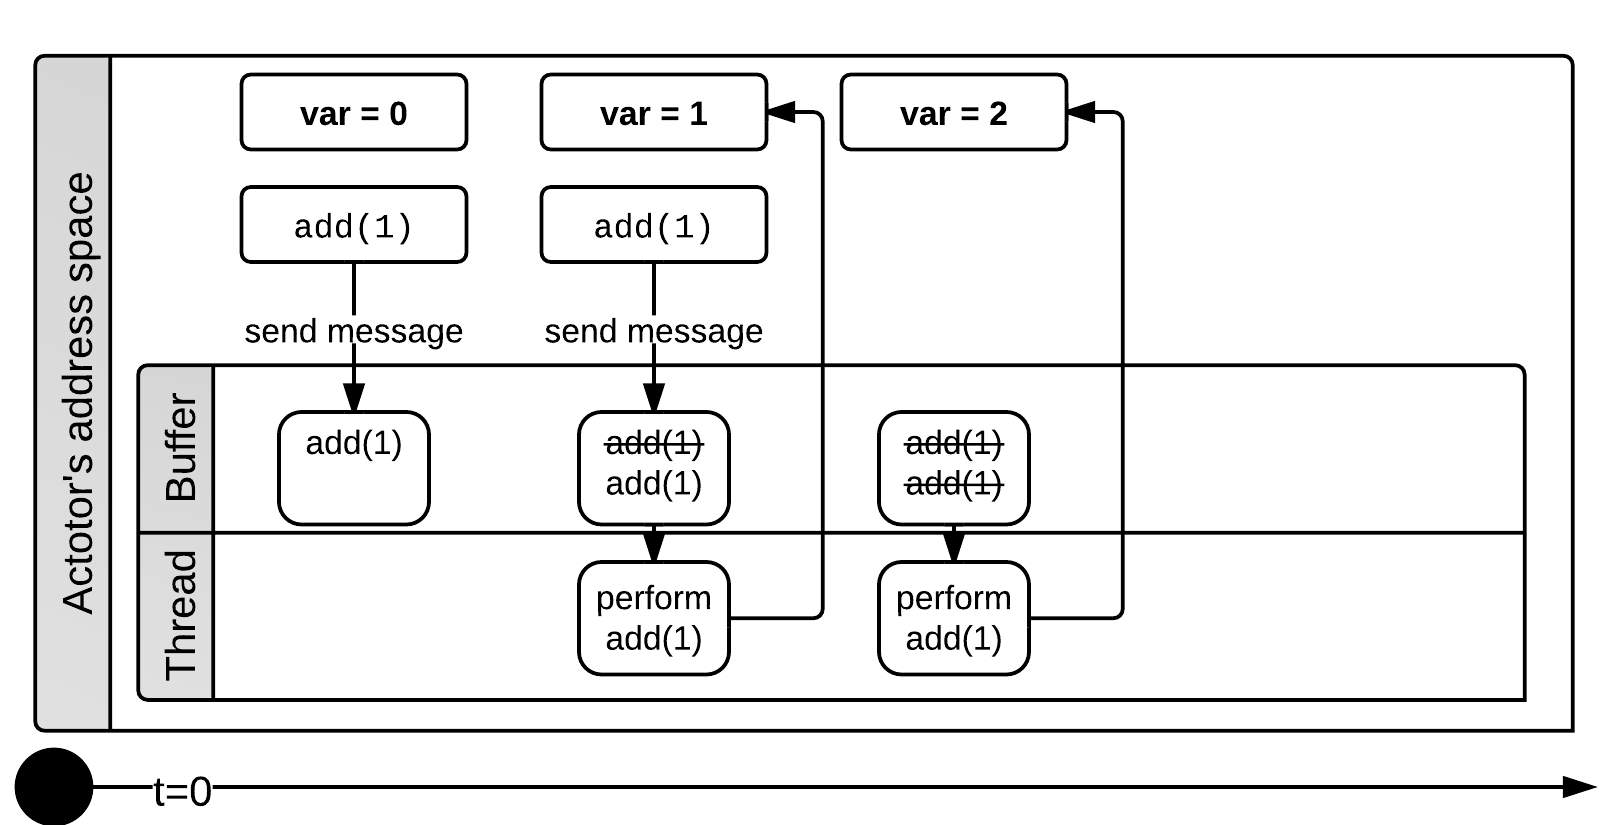
\includegraphics{images/ActorsAdd.png}
    \end{center}
    \caption{Asynchronous message passing between Actors.}
    \label{fig:actorsAdd}
\end{figure}

\section{Simulation}

Now that we have defined our three actions: \texttt{deposit}, \texttt{withdraw} and \texttt{transfer}, we can use them to build a simple simulation in which multiple actors, each with their own balance, transfer funds between each other. 

The constraints of the simulation are the following:

\begin{enumerate}
\item Actors must be able to transfer money between each other of their own accord.
\item The simulation must end.
\item The total amount of money in the system must be the same at the beginning and end of the simulation.
\end{enumerate}

The second constraint guards against deadlock, which as we will see is still possible in an actor system.

The final constraint is our (informal) proof of correctness - if the amount of money in the system remains the same then we can be fairly sure that money is not generated or lost through errors arising from race conditions. \\

Actor-based systems can be implemented in many JVM languages, but usually through third-party libraries such as the Akka library \footnote{http://akka.io/}. In this section, we will use the language Groovy, which includes the GPars concurrency toolkit as part of its standard library.

\section{A naive version}

Our first implementation of the simulation tries to keep the system as simple as possible. We define just the one Actor - called Person - that has a name and a balance as its state. This Person accepts two messages, \texttt{Deposit} and \texttt{Withdraw} that affect this state. 

\subsection{Messages}
Below is an example implementation of an immutable message that Actors use to communicate between each other. The message is \textbf{not} subject to change which preserves that the received message is not altered after it has been sent.

\begin{listing}[H]
	\begin{minted}[linenos=true,bgcolor=code]{java}
class Person extends DefaultActor {
    final class Deposit { float amount }
    final class Withdraw { float amount }
    ...
}
	\end{minted}
\end{listing}

A common idiom in generally mutable, object oriented languages is to explicitly define messages as immutable classes, as we do here with the \texttt{final} keyword. A problem with this approach is that forgetting to declare a message as \texttt{final}, and then accidentally mutating it, can result in very subtle bugs.

The \texttt{Person} actor handles these incoming messages as follows:

\begin{listing}[H]
	\begin{minted}[linenos=true,bgcolor=code]{java}
def handle(message) { 
    switch(message) {
        case Deposit:
            reply deposit(message.amount)
            break
        case Withdraw: 
            reply withdraw(message.amount)
            break
    }
}
	\end{minted}
\end{listing}

A very obvious issue with this message handling code is how redundant it is: messages containing data call the corresponding functions on the actor with their data transformed to arguments. As we see in later sections, this actor boilerplate code can and should be abstracted away.

\subsection{Actions}

Let's see how our actions look:

\begin{listing}[H]
	\begin{minted}[linenos=true,bgcolor=code]{java}
boolean deposit(float amount) {
    balance += amount
    say "Deposited $amount, balance is now $balance"
    return true
}

boolean withdraw(float amount) {
    if (balance - amount >= 0) {
        balance -= amount
        say "Withdrew $amount, balance is now $balance"
        return true
    } else {
        say "That's more than I have!!"
        return false
    }
}

void transfer(Person target, float amount) {
    say "Sending $amount to $target"
    def success = withdraw(amount)
    if (success) { 
        target.sendAndWait new Deposit(amount: amount)
    } 
}
	\end{minted}
\end{listing}

A refreshing feature of this code is the lack of locking boilerplate around the \texttt{balance} instance variable. We are allowed to leave \texttt{balance} lock-free because of the semantics of the actor model - by definition, only one message, and therefore action, can be processed at any one time. This makes each action atomic and means we do not have to worry about shared memory related race conditions within the actions themselves.

\subsection{Deadlock}

That said, our naive implementation does suffer from quite an extreme bug, which we can see from the code that handles each Person's lifecycle (this is an Actor's equivalent to \texttt{Thread\#run}):

\begin{listing}[H]
	\begin{minted}[linenos=true,bgcolor=code]{java}
void act() {
    loop {
        int amount = Math.random()*50
        transfer(world.randomOther(this), amount)
        react { message -> handle(message) }
    }
}
	\end{minted}
\end{listing}

Like with our earlier transfer implementation, this can lead to deadlock in the following scenario:

\begin{enumerate}
\item Person A begins a transfer to Person B
\item Person A: \texttt{personB.sendAndWait new Deposit(amount: amount)}
\item Person B begins a transfer to Person A
\item Person B: \texttt{personA.sendAndWait new Deposit(amount: amount)}
\end{enumerate}

\texttt{sendAndWait} is a \textbf{synchronous} operation, i.e. it blocks the actor until it receives a reply, which in this case would be a \texttt{boolean} indicating whether the deposit succeeded.

Unfortunately for Persons A and B, they will wait forever, as they are waiting on each other so neither Person will complete their \texttt{transfer} method call and be able to process the incoming \texttt{Deposit} message inside \texttt{react}.

This illustrates one of the biggest pitfalls of actor-based systems: as soon as synchronous messages are included within an actor's logic, there is the risk of deadlock. We could solve this problem by allowing \texttt{sendAndWait} to time out, or by making it an asynchronous message, but these seem like workarounds for a badly designed system. In the next section, we will instead rethink our actors and messages to try and eliminate this problem.

\section{Introducing brokers}

It seems that we gave our Person actors a little too much responsibility in our first implementation. Allowing them to handle \texttt{Withdraw} and \texttt{Deposit} messages seems natural, but when we made them handle transfers themselves we ran into trouble.

In this version of the simulation we will introduce a new actor, called a \texttt{Broker}, that has the sole purpose of handling transfers between Persons. By extracting the transfer logic from the Person class, we allow Persons to simply \texttt{react} to \texttt{Withdraw} and \texttt{Deposit} messages, thereby eliminating our case of deadlock. 

\begin{figure}[H]
    \begin{center}
    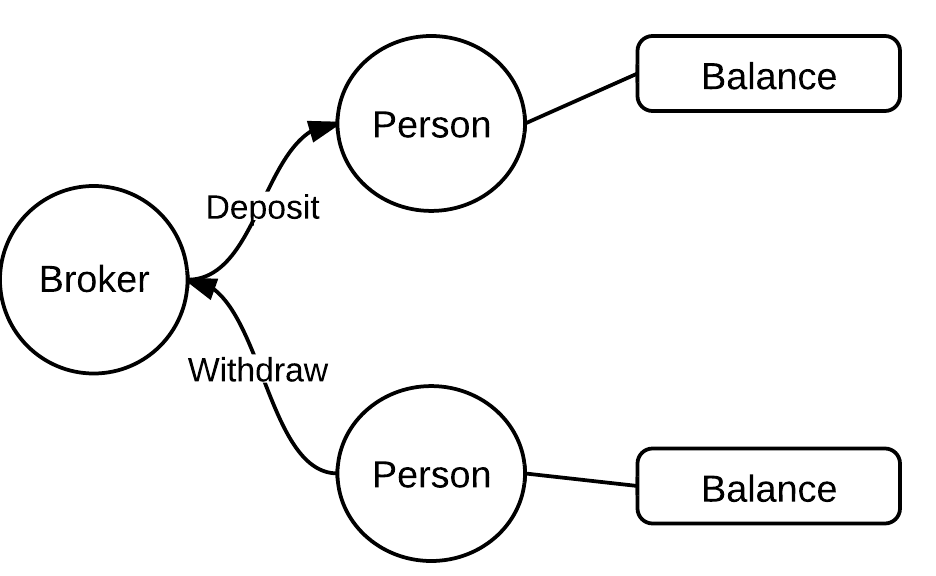
\includegraphics{images/ActorsBroker.png}
    \end{center}
    \caption{A Broker coordinates messages to prevent deadlocks.}
    \label{fig:actorsBrooker}
\end{figure}

\subsection{Messages}

\begin{listing}[H]
	\begin{minted}[bgcolor=code]{java}
final class TransferRequest { def from; def to; float amount }
	\end{minted}
\end{listing}

\subsection{Actions}

\begin{listing}[H]
	\begin{minted}[linenos=true,bgcolor=code]{java}
class Broker extends AccountActor {
    void transfer(from, to, float amount) {
        say "Sending \$amount from \$from to \$to"
        def success = 
            from.sendAndWait new Withdraw(amount: amount)
        if (success) { 
            to.sendAndWait new Deposit(amount: amount) 
        } 
    }

    void act() {
        loop {
            react { 
                switch(it) {
                    case TransferRequest:
                        transfer(it.from, it.to, it.amount)
                        break
                }
            }
        }
    }
}
	\end{minted}
\end{listing}

It is pretty obvious here that the \texttt{Broker} actor exists simply to wrap the \texttt{transfer} method. 

Now we have an extra \texttt{sendAndWait} call for the withdrawal. This time however, the risk of the same kind of deadlock as earlier is eliminated, due to the simplification of \texttt{Person}'s act loop:

\begin{listing}[H]
	\begin{minted}[linenos=true,bgcolor=code]{java}
class Person extends AccountActor {
    ...
    void act() {
        loop { react { message -> handle(message) } }
    }
    ...
}
	\end{minted}
\end{listing}

Because \texttt{Person} is now purely reactive - it has no other logic in \texttt{act} than \texttt{react} - there is no chance that a Person will not be able to respond to messages from a \texttt{transfer}. This in turn means our two \texttt{sendAndWait}s in \texttt{transfer} should not cause deadlock.

\subsection{Autonomous Actors}

But where in \texttt{Person} is a transfer actually instigated? Although we now fulfil the second constraint of our simulation (no deadlock), how can we fulfil the first (that Persons transfer money between each other) while still keeping \texttt{Person} fully reactive?

The solution is not immediately apparent. Generally we are used to objects, that, like our new actors, simply react to messages or method calls. These objects tend not to execute code on their own accord. 

As always when we require code to be executed asynchronously, the answer lies in spawning more threads. If we would like transfers to be made every few seconds, which does make for a more realistic simulation, we could use a Java \texttt{ScheduledThreadPoolExecutor}. This object allows us to schedule a block of code to be executed periodically, on a Thread pool it manages itself.

This sounds good until we realise that by allowing code running on a thread managed by a \texttt{ScheduledThreadPoolExecutor} to execute methods within our actors, we break the very semantics of the Actor model, which state that only the appropriate \texttt{Actor thread} may execute an actor's methods. Clearly this is not something we want to do as it would return us to a shared, mutable state scenario which would require us to again think about race conditions.

One solution, called \textit{murmurs} by Venkat Subramaniam, is to have this scheduled thread make an actor send a message to \textit{itself}. This has the effect of adding an action to the actor's queue, which, crucially, will eventually be executed by the \texttt{Actor thread}, not the scheduled thread. In this way, we preserve the semantics of the Actor model, and allow actors to remain fully reactive: now they simply need to react to an extra message that they send to themselves.

\begin{listing}[H]
	\begin{minted}[linenos=true,bgcolor=code]{java}
class Person extends AccountActor {
    ...
    static ScheduledThreadPoolExecutor timer = 
        new ScheduledThreadPoolExecutor(2)

    void requestTransfer() {
        int amount = Math.random()*100
        def target = world.randomMember(this)
        def broker = world.getBroker()
        broker?.send 
            new TransferRequest(from: this, 
            to: target, amount: amount)
    }

    def handle(message) { 
        switch(message) {
            case Start:
                say "Starting"
                timer.scheduleAtFixedRate(
                    { send new Tick() },
                    0, 100, TimeUnit.MILLISECONDS
                )
                break
            case Tick:
                requestTransfer()
                break
            case Deposit:
                reply deposit(message.amount)
                break
            case Withdraw: 
                reply withdraw(message.amount)
                break
        }
    }
    ...
}
	\end{minted}
\end{listing}

This pattern of using \textit{murmurs} to make fully reactive actors autonomous is a powerful one, and it would be a shame to have to implement it from scratch every time we want a ticking actor. Similarly, having to create messages and write handlers purely to call the appropriate method with the appropriate arguments is getting quite monotonous, so our next section will deal with how to abstract away a lot of the Actor boilerplate, resulting in far cleaner code.

\section{Active Objects}

Active Objects are an object-oriented facade over the Actor model. Every Active Object instance has its own hidden actor, and whenever certain methods, called Active Methods, are called on these Active Objects, the method call is translated to a message that is passed to this hidden actor.

What this means is that we can scrap the entirety of our message handling boilerplate while retaining the semantics of having only one thread inside an Active Method at one time. Also, as methods are no longer coupled to a message handling routine, we can distribute them across objects using standard inheritance.

For example, we can now extract the ticking logic from \texttt{Person} into the more general \texttt{TickingActor} class:

\begin{listing}[H]
	\begin{minted}[linenos=true,bgcolor=code]{java}
@ActiveObject
abstract class TickingActor extends NamedActor {
    static final TIMER_THREADS = 2
    static final ScheduledThreadPoolExecutor TIMER = 
        new ScheduledThreadPoolExecutor(TIMER_THREADS)

    static TIMER_INTERVAL = 100
    static TIMER_INTERVAL_UNIT = TimeUnit.MILLISECONDS

    TickingActor() {
        TIMER.scheduleAtFixedRate(
            { this.tick() },
            0, TIMER_INTERVAL, TIMER_INTERVAL_UNIT
        )
    }

    abstract void tick();
}
	\end{minted}
\end{listing}	

Here we can see that \texttt{this.send new Tick()} has become simply \texttt{this.tick()}, and we can use Java's usual \texttt{abstract} semantics to signify that concrete child classes must implement the \texttt{tick} method.

Our \texttt{Person} class becomes similarly simplified, leaving us with just the logic that is specific to a Person and its state.

\begin{listing}[H]
	\begin{minted}[linenos=true,bgcolor=code]{java}
@ActiveObject
class Person extends TickingActor {
    ...
    @ActiveMethod(blocking=true)
    boolean deposit(float amount) {
        balance += amount
        say "Deposited $amount, balance is now $balance"
        return true
    }

    @ActiveMethod(blocking=true)
    boolean withdraw(float amount) {
        if (balance - amount >= 0) {
            balance -= amount
            say "Withdrew $amount, balance is now $balance"
            return true
        } else {
            say "That's more than I have!!"
            return false
        }
    }

    @Override
    @ActiveMethod
    void tick() {
        int amount = Math.random()*100
        def target = world.randomMember(this)
        def broker = world.getBroker()
        broker?.transfer(this, target, amount)
    }
}
	\end{minted}
\end{listing}	

\section{Problems}

We've made a lot of progress with Actors, going from a deadlocking, broken Actor system to a streamlined, reusable system using Active Objects. Nevertheless, our implementation still suffers from some drawbacks.

\subsection{Read performance}

If we were to replace our \texttt{@ActiveMethod} decorators with the \texttt{synchronized} keyword, the semantics of our objects would barely change. Like with the most primitive form of locking, reads will be serialised as well as writes in an Active Object, as after all they are just responses to messages. That said, it can be argued that Active Objects are simpler to reason about than \texttt{synchronized} locking, and as we are using higher-level constructs it is entirely possible for read performance to be optimised in the Active Object implementation without any changes required in our code.

\subsection{Actors vs Threads}

We also gain by using the higher-level Actor abstraction as opposed to threads. Though the Actor model requires that only one thread execute methods within an Actor at one time, there is no requirement that it is the \textit{same} thread. As a result, we can easily have a crowd of Actors sharing a limited pool of threads, where the thread pool size is optimised for the number of available processors. 

Again this could be achieved using \texttt{Executors} and locking, and indeed it probably is in the underlying Actor implementation, but if a library exists it should be used instead of writing our own code.

\subsection{Transactions}

One of the last problems with our implementation is that our simulation is still quite fragile. If a Person instance dies mid-transfer, then the Broker carrying out the transfer will deadlock and the amount of money in the system will be inconsistent.  Also, the return of a boolean signifying whether an action succeeded is not as semantic as it could be: for example if a message is never received, \texttt{False} will never be returned and hence a \texttt{MessageNotReceivedException} is more appropriate.

In these cases, we would like failed transfers to behave like \textit{transactions}, i.e. they should be rolled back on failure, leaving no trace of their execution, so they can be retried at a later time. This is possible using a system known as Software Transactional Memory (STM), which we will discuss next.

\part{ Software Transactional Memory}

\section{Background}
Software transactional memory (STM) is influenced by database transactions and that operations are conceptually \textbf{atomic}. STM provides abstraction of handling in-code synchronisation and provide the appearance that code is executed sequentially. Every transaction maintains a log to track its progress in case it would be \textit{aborted} to enable the operations to be \textit{rolled back}. If the transaction was successful the operations is \textit{commited} and changes made permanent.

STM enables composition of atomic operations\cite{cmt} which is hard to achieve in tradtional lock-based programs. This proves extremely useful to avoid inconsistency when executing two dependent operations.

\section{Concurrency in Clojure}
Clojure is the third JVM language we will use. Unlike the object-oriented Java and Groovy, Clojure is a functional language that also happens to be a dialect of LISP.  Consequently, Clojure tries to avoid shared, mutable objects and focuses instead on immutable data structures and functions that operate on them.

Clojure provides a separation of state and identity, where an identity could be viewed as an account and the the balance the state. A withdrawal does not change the identity rather it affects its state. The balance prior the withdrawal becomes a record of the balance at that time and that state is immutable. In Clojure all values and collections are, by design, \textbf{immutable} and an identity could only change state in a \textbf{transaction}.

The use of operations with side effects in transactions is highly discouraged due to difficulties to perform rollback \footnote{\url{http://clojure.org/refs}}. For example I/O-operations could prove extremely hard to redo and printing to e.g. a log could obfuscate it. Best practice is to schedule operations with side effects in a post-commit section.

MVCC tag the data with a read and write timestamp to keep track of the current version. When a write transaction $T_i$ is started the latest version of the data is available as a snapshot with a timestamp $TS(T_i)$. If another write transaction $T_j$ is running, there must exist a timestamped version $TS(T_j)$ where $TS(T_i) \lt TS(T_j)$ to complete and for $T_i$ to commit. Otherwise $T_i$ is aborted and any changes rollbacked. This ensures consistency as well as isolation since each transaction work with its own snapshot.

\begin{figure}[H]
\centering
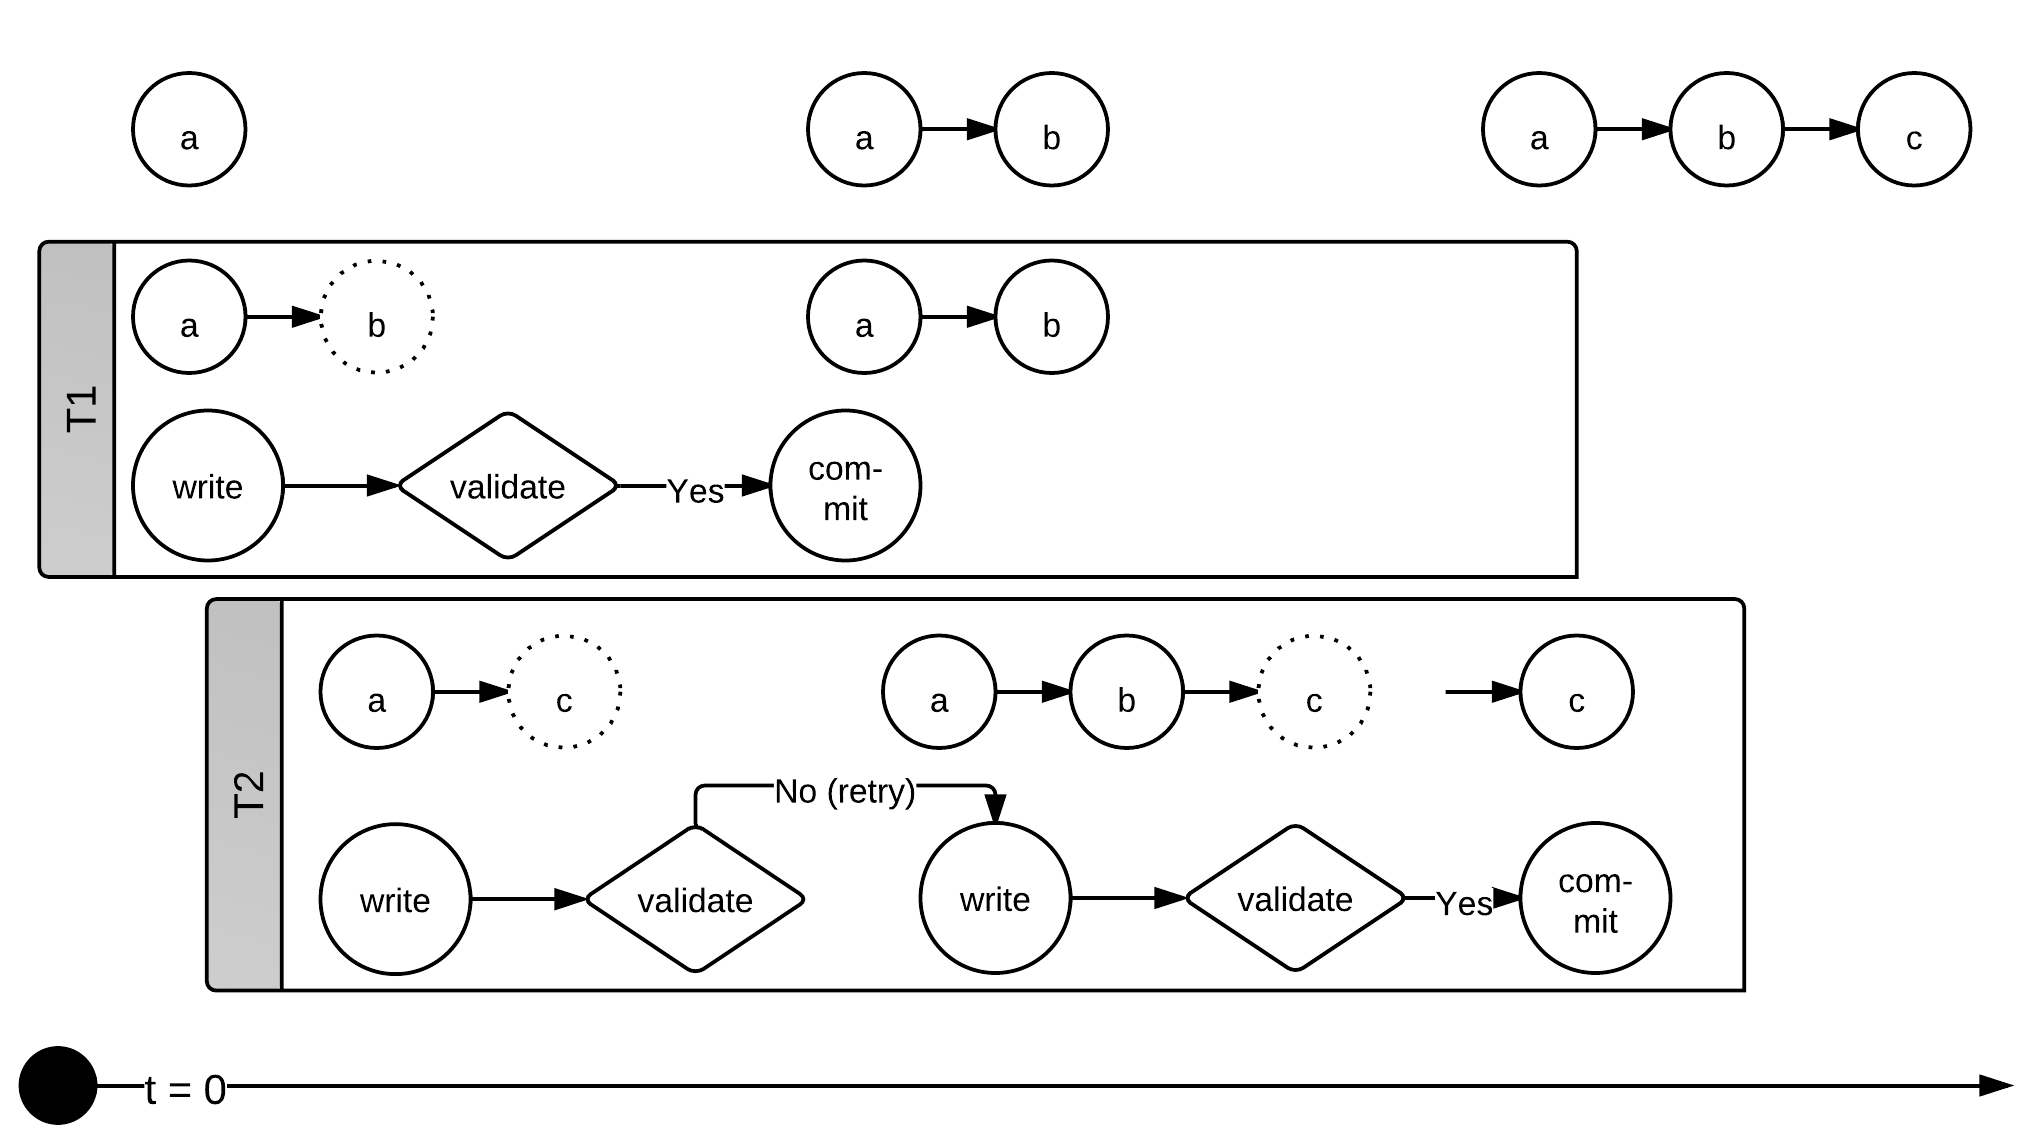
\includegraphics[scale=0.8]{images/TransactionWriteCollision.png}
\caption{A write collision when inserting element in a linked list}
\label{fig:twc}
\end{figure}

Looking at the illustration Figure~\ref{fig:twc} of a write collision that occur when $T_2$ tries to insert an element before $T_1$ has successfully commited, $T_2$ silently aborts and retry the insert operation with a fresh snapshot reflecting the changes made by $T_1$.

\section{Immutable data types}

Data types are immutable by default, which we can see in the following snippet executed in the Clojure REPL:

\begin{listing}[H]
	\begin{minted}[linenos=true,bgcolor=code]{clojure}
user=> (def x 1)
#'user/x
user=> x
1
user=> (inc x)
2
user=> x
1
	\end{minted}
\end{listing}

Instead of \textit{assigning} 1 to the variable \texttt{x}, we \textit{define} it to be 1. Executing the increment function with \texttt{x} as an argument results in a new value 2 and leaves \texttt{x} unchanged.

This makes reasoning about programs a lot easier as equality is not subject to change, and the effects of sharing data with other threads or even other modules is a lot more predictable when that data is immutable.

\section{Mutable reference types}

However, there are times when mutable data can be very useful. Clojure has three reference types that act as 'wrappers' for data structures. These wrappers ensure that changes to these references are protected against a lot of problems usually associated with mutable state change.

\subsection{Atoms}

The simplest of these types is called an \texttt{atom}. Atoms are references to data that facilitate \textbf{uncoordinated}, \textbf{synchronous} changes to their value. This is how they look in action:

\begin{listing}[H]
	\begin{minted}[linenos=true,bgcolor=code]{clojure}
user=> (def x (atom 1))
#'user/x
user=> x
#<Atom 24e33e18: 1>
user=> (swap! x inc)
2
user=> x
#<Atom 24e33e18: 2>
	\end{minted}
\end{listing}

This time we used the \texttt{swap!} function to \textbf{atomically} swap the current value of \texttt{x} for the value returned after executing the increment function. This change was synchronous (it happened immediately) and uncoordinated (it was independent of other actions).

Though this may have added a little additional complexity to dealing with data - we have to use \texttt{swap} to change a reference's value instead of executing functions directly - we gain massive benefits when atoms are shared between threads:

\begin{listing}[H]
	\begin{minted}[linenos=true,bgcolor=code]{clojure}
(defn sleepy-inc [a]
    (Thread/sleep 1)
    (inc a))

(defn inc-atom! []
    (let [x (atom 0)]
        (println "x: " @x)
        (do-pool! 10
            (fn [pool]
                (dothreads! 
                    #(swap! x sleepy-inc) 
                    pool :threads 10 :times 1)))
        (println "x: " @x)))
        
accounts=> (inc-atom!)
x: 0
x: 10
nil
	\end{minted}
\end{listing}

Here we define \texttt{x} as an atom with the initial value of 0. We then increment \texttt{x} 10 times from 10 different threads, simultaneously (context switches are forced by the \texttt{Thread/sleep} in \texttt{sleepy-inc}). When these threads are all done, we check the value of \texttt{x} with the dereference macro, @, and see that its value is 10 as expected.

\subsection{Validators}

We can see mutable references as state machines, with the value of a reference being its state and transitions being the functions supplied to \texttt{swap!}. These functions take the current state of the reference as input, and return the next state as output. 

An effect of this paradigm is that data structures are kept strictly separated from the functions that act on them, unlike Object Oriented Programming where state is stored in an objects instance variables and functions that act on them make up its instance methods.

Whenever functions, or methods, operate on data there is a risk of the object or data structure finding itself in an invalid state. A familiar example for us is a reference representing a balance, where a negative balance is invalid. A sensible place to store information about valid and invalid states is with the data itself, not the functions that operate on it.

For us this would mean storing information about a balance validity with the balance \textit{reference} itself, not within the functions that act on it. We do this by using \texttt{set-validator!}:

\begin{listing}[H]
	\begin{minted}[linenos=true,bgcolor=code]{clojure}
user=> (def balance (atom 10))
#'user/balance
user=> (set-validator! balance #(>= % 0)) 
nil
user=> (swap! balance - 10)
0
user=> @balance
0
user=> (swap! balance - 1)
IllegalStateException Invalid reference state
user=> @balance
0
	\end{minted}
\end{listing}

In line 3 we declare that \texttt{balance} is only valid if the form \texttt{(>= \% 0)} returns true, with the \texttt{\%} being replaced by  the value of a new state. If the validator fails then we get an \texttt{IllegalStateException} and \texttt{balance} remains at its old, valid, state.

\subsection{Refs}

Now We have seen how validators work, let's get back to Clojure's reference types.

Sometimes changes to multiple mutable references needs to be coordinated. For these cases we wrap data types with reference types called \texttt{ref}. We can change the value of a \texttt{ref} using \texttt{alter}, which, like \texttt{swap!}, sets the new value of a \texttt{ref} to that returned by the supplied function. 

\begin{listing}[H]
	\begin{minted}[linenos=true,bgcolor=code]{clojure}
user=> (def x (ref 1))
#'user/x
user=> x
#<Ref@4826dfcc: 1>
user=> (alter x inc)
IllegalStateException No transaction running
	\end{minted}
\end{listing}

Here we can see what coordinated change really means. An exception was thrown because we tried to \texttt{alter} a \texttt{ref}'s value \textbf{independently}. Instead, \texttt{ref}s are meant to be used within \textbf{transactions}, as part of Clojure's Software Transactional Memory implementation. 

\subsection{Transactions}
Database transactions obey to atomicity, consistency, isolation and durability\footnote{In concurrency control this is known under the acronym ACID} and for transactions in Clojure the first three are valid. Durability is not an issue since values are stored in volatile memory (RAM).

\begin{description}
    \item[Atomicity] The transaction was successful or did not happen. This prevents race-conditions to occur.
    \item[Consistency] The data integrity is maintained after transaction is executed regardless if commit or aborts the result. In case of two simultaneous \texttt{withdraw} and \texttt{deposit} the balance correctly reflects the yielded result from both operations.
    \item[Isolation] Transition states are not visible to other transactions, only the outcome of an success becomes visible for other transactions.
\end{description}

The use of operations with side effects in transactions is highly discouraged due to difficulties to perform rollback\footnote{\url{http://clojure.org/refs}}. For example I/O-operations could prove extremely hard to redo and printing to e.g. a log could obfuscate it. Best practice is to schedule operations with side effects in a post-commit section.

MVCC tag the data with a read and write timestamp to keep track of the current version. When a write transaction $T_i$ is started the latest version of the data is available as a snapshot with a timestamp $TS(T_i)$. If another write transaction $T_j$ is running, there must exist a timestamped version $TS(T_j)$ where $TS(T_i) \lt TS(T_j)$ to complete and for $T_i$ to commit. Otherwise $T_i$ is aborted and any changes rolled back. This ensures consistency as well as isolation since each transaction work with its own snapshot.

\begin{figure}[H]
\centering
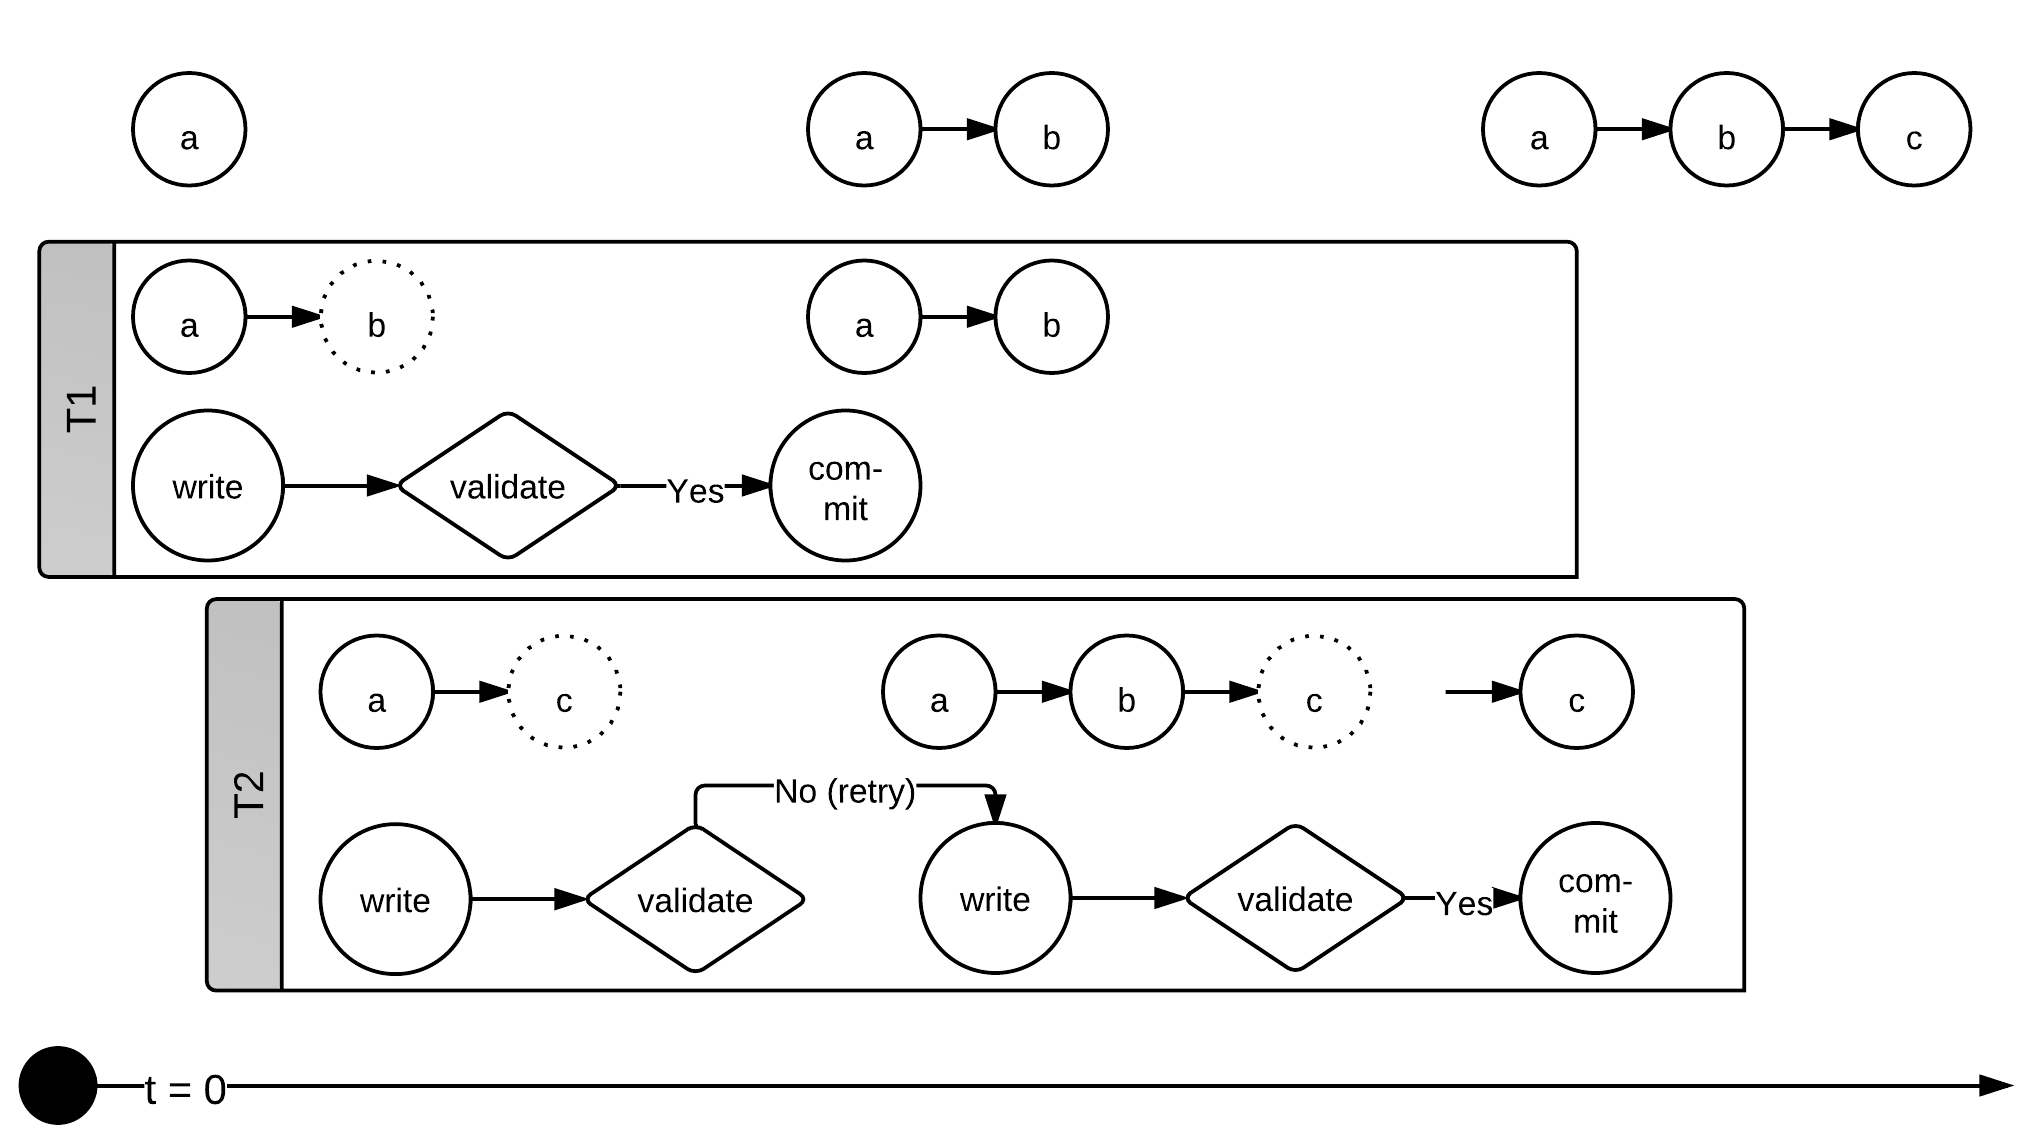
\includegraphics[scale=0.8]{images/TransactionWriteCollision.png}
\caption{A write collision when inserting element in a linked list.}
\label{fig:twc}
\end{figure}

Looking at the illustration Figure~\ref{fig:twc} of a write collision that occurs when $T_2$ tries to insert an element before $T_1$ has successfully commited, then $T_2$ silently aborts and retries the insert operation with a fresh snapshot reflecting the changes made by $T_1$.

A transaction is delineated by the \texttt{dosync} form:

\begin{listing}[H]
	\begin{minted}[linenos=true,bgcolor=code]{clojure}
user=> (dosync (alter x inc))
2
user=> x
#<Ref@4826dfcc: 2>
	\end{minted}
\end{listing}

Transactions reveal their usefulness when we consider how they allow us to coordinate changes to multiple \texttt{ref}s all with their own validators.

For example, let's define a donate function that takes a donor and a receiver, and transfers 1 unit from the donor to the receiver.

\begin{listing}[H]
	\begin{minted}[linenos=true,bgcolor=code]{clojure}
(defn donate [donor receiver]
    (dosync 
        (alter receiver inc)
        (alter donor dec)))
	\end{minted}
\end{listing}

By wrapping these \texttt{alters} in \texttt{dosync} we declare that \texttt{donate} is a transaction: either the \texttt{inc} \textit{and} the \texttt{dec} should \textit{both} succeed, or the entire operation should be rolled back as if it never happened. 

We can take \texttt{donate} for a test run with the following function:

\begin{listing}[H]
	\begin{minted}[linenos=true,bgcolor=code]{clojure}
(defn mk-balance [b]
    (let [balance (ref b)]
        (set-validator! balance #(>= % 0))
        balance))

(defn donation [donor-balances]
    (let [donors (map mk-balance donor-balances)
          receiver (mk-balance 0)]
        (doseq [d donors]  
            (try 
                (donate d receiver)
                (catch IllegalStateException e)))
        (println "donors:" donors)
        (println "receiver:" receiver)))
	\end{minted}
\end{listing}

All is well when the donors have money to give:

\begin{listing}[H]
	\begin{minted}[linenos=true,bgcolor=code]{clojure}
accounts=> (donation [10 10 10])
donors: (#<Ref@751201a1: 9> #<Ref@71292d12: 9> 
#<Ref@464e32c8: 9>)
receiver: #<Ref@69ce835b: 3>
	\end{minted}
\end{listing}

Each donor donated 1 to the receiver, leaving the donors with 9 each and the receiver with 3.

But what happens if one of the donors is in fact as poor as the receiver, and has nothing to give?

\begin{listing}[H]
	\begin{minted}[linenos=true,bgcolor=code]{clojure}
accounts=> (donation [10 0 10])
donors: (#<Ref@2f6e4ddd: 9> #<Ref@72ba007e: 0> 
#<Ref@11768b0a: 9>)
receiver: #<Ref@7e349a0e: 2>
	\end{minted}
\end{listing}

Surprisingly enough, nothing broke! Because \texttt{donate} is a transaction, when the time came for the donor with the empty balance to donate, the \texttt{IllegalStateException} thrown by the \texttt{dec} to the donor caused the whole transaction to fail and the \texttt{inc} to the receiver's balance was not committed. As a result, the system remained consistent.

\subsection{Agents}

Agents are for \textit{potentially} coordinated, \textbf{asynchronous} change to mutable references. Instead of replacing state with the results of \texttt{alter} or \texttt{swap!}, we affect agents by \texttt{send}ing them state-transition functions. These functions are queued and executed asynchronously on the agent's own thread. We can see this in action here:

\begin{listing}[H]
	\begin{minted}[linenos=true,bgcolor=code]{clojure}
(defn time-agent [times sleep]
    (let [x (agent 0)]
        (dotimes [_ times]
            (send-off x
                (fn [x]
                    (Thread/sleep sleep)
                    (inc x))))
        (time (await x))
        @x))
        
accounts=> (time-agent 1 1000)
"Elapsed time: 1001.424 msecs"
1
accounts=> (time-agent 2 1000)
"Elapsed time: 2002.785 msecs"
2
	\end{minted}
\end{listing}

We send an agent a number of anonymous functions that cause it to sleep and then increment its value. We then time how long it takes for the agent to process its queue. After running \texttt{time-agent} the time taken indicates that these sent functions are indeed executed sequentially.

\subsection{Actors vs Reference types}

On the surface, Clojure's agents seem very similar to Groovy's actors: both allow asynchronous change of state guaranteed to take place on a single thread. Nonetheless, they do differ in some key areas.

\subsubsection{Read performance}

Retrieving the value of an agent, or any reference type, does not require us to send it a message. 

\begin{listing}[H]
	\begin{minted}[linenos=true,bgcolor=code]{clojure}
accounts=> (send-off x (fn [x] (Thread/sleep 10000) (inc x)))
#<Agent@127e942f: 0>
accounts=> @x ; Immediately
0
accounts=> @x ; 10 seconds later
1
	\end{minted}
\end{listing}

Not only does this show that agents are indeed asynchronous, but we also see that we can dereference them to get their value while they are processing messages, in constant time.

This is a result of Clojure's reference type semantics - we do not need to use a function to get an agent's value as functions are solely for state transitions, which is not what a read-value-function represents. Instead, as reference types are designed to be state machines, dereferencing can be supported as a ''special case'' operation for returning a machine's current state.

\subsubsection{Flexibility}

Unlike with actors, the set of possible messages you can send a reference type is open. As we have demonstrated, it is entirely possible to send, swap or alter a reference type with an anonymous function, something that would be impossible if we had to define messages and methods in advance. This lack of boilerplate makes Clojure reference types both more concise and more extensible than Actors.

\section{Simulation 2.0}

Now that we have been introduced to Clojure's approach to concurrency, we can try to rethink our simulation to fit these patterns. These patterns have very strict semantics so we should take care not to violate them.

\subsection{Rethinking brokers}

Brokers as a middleman actor seemed a good idea at the time, as they removed a potential deadlock from our system and allowed all actors to simply react. However, a facet of Brokers that was easy to miss in Groovy but is painfully obvious in Clojure is that they are \textbf{stateless}. Therefore, we should avoid implementing them as agents in Groovy as this would break our state-machine semantics.

\subsection{Rethinking people}

Making a Person a type of Actor made sense in Groovy, but that was in a language in which state and behaviour are not clearly distinguished. In Clojure, we can see clearly that a Person is simply a custom data type that we can define like this:

\begin{listing}[H]
	\begin{minted}[bgcolor=code]{clojure}
(defrecord Person [name balance])
	\end{minted}
\end{listing}

We can think of a Person as a record with fields for a name and a balance. This is a pure declaration of state; definitions of behaviour are stored in the functions that act on these records.

\subsection{Transfers are synchronous}

In our Groovy implementation, we used \texttt{sendAndWait} (and later a blocking \texttt{ActiveMethod}) in our transfers that made them wait until the \texttt{withdraw} and \texttt{deposit} completed before returning. In the context of our simulation, where all we do is transfer (as we do not want to generate or lose money), having \texttt{withdraw} and \texttt{deposit} as asynchronous actions does not make sense. And if we do not need asynchronous actions, maybe we shouldn't be using agents at all.

\subsection{Choosing a reference type}

So what should we use if not agents? We have established that our transitions (\texttt{withdraw} and \texttt{deposit}) need to be \textbf{synchronous} and \textbf{coordinated}. The Clojure reference type for that is a \texttt{ref}. We can write a kind of factory method for these reference types that creates the underlying record, wraps it and sets the appropriate helper functions.

\begin{listing}[H]
	\begin{minted}[linenos=true,bgcolor=code]{clojure}
(defn make-person [name balance]
    (let [person (ref (Person. name balance))]
        (set-validator! person 
            (fn [new-state] (>= (:balance new-state) 0)))
        (add-watch person :print-balance
            (fn [k p old-state new-state] 
                (let [n (:name new-state)
                      b1 (:balance old-state)
                      b2 (:balance new-state)]
                    (println n ": balance" b1 "->" b2))))
        person))
	\end{minted}
\end{listing}

Here we declare what a valid state should look like, and also add a watcher function that will be called whenever the Person's state changes. Again, these functions are purely concerned with issues of state, and it feels far cleaner to declare them here once instead of having to validate and fire our own watchers in every instance method as we would have to in an object oriented language.

\subsection{Rethinking autonomy}

Whatever changes we make, we must ensure that we maintain our core idea of simulating transfers between autonomous entities. Even though our ticking actors with their murmurs seemed a good solution for this, we can see now that murmurs were actually a workaround for Actor semantics (only one thread in an actor's body), and we know now we shouldn't have been using actors at all.

We can simplify matters by realising that we can simulate autonomy by scheduling a repeating function \texttt{f} that represents the actions of a single person. If we schedule this function for every Person in our simulation then we can say that every Person is acting autonomously.

\begin{listing}[H]
	\begin{minted}[linenos=true,bgcolor=code]{clojure}
(def TICK-INTERVAL 100) 
(defn start [me people timeline]
    (schedule
        (fn [] 
            (let [target (rand-other people me)
                  amount (rand-int 100)]
                (try 
                    (transfer me target amount)
                    (println "Transferred" amount 
                        "from" me "to" target)
                    (catch IllegalStateException e))))
        timeline TICK-INTERVAL))
	\end{minted}
\end{listing}

That function \texttt{f} is the anonymous function on line 4. In fact, it is a closure that closes over the variable \texttt{me}, which represents the Person we are starting. In this way this function represents a Person's ''unique'', autonomous behaviour. 

This behaviour is scheduled on the given timeline, which, like in Groovy, is a \texttt{ScheduledThreadPoolExecutor}. The difference is that it is entirely okay for the scheduled thread to actually do the transfer - we do not need the added complexity of handing execution back to an actor thread any more.

\subsection{Rethinking actions}

We can do this because of how we implement \texttt{transfer}, \texttt{withdraw} and \texttt{deposit}.

\begin{listing}[H]
	\begin{minted}[linenos=true,bgcolor=code]{clojure}
(defn transfer [sender receiver amount]
    (dosync
        (deposit receiver amount)
        (withdraw sender amount)))

(defn deposit [person amount]
    (dosync
        (let [balance (:balance @person)]
        (alter person assoc :balance (+ balance amount)))))

(defn withdraw [person amount]
    (dosync
        (let [balance (:balance @person)]
        (alter person assoc :balance (- balance amount)))))
	\end{minted}
\end{listing}

Finally we define some behaviour to go with our state. As we can see, we only have logic that is specific to the action; validation and monitoring of state is handled by our helper functions that were defined earlier.

Every action is wrapped in a transaction, as transactions can nest without issue. The fact that \texttt{withdraw} and \texttt{deposit} are transactions ensures that withdrawals and deposits on the same Person do not conflict; the fact that \texttt{transfer} is a transaction ensures that its effects are committed iff both the \texttt{deposit} and \texttt{withdraw} \textit{both} succeed. The \texttt{transfer} function is a perfect example of \textbf{composed operations} and it is for this reason we can safely deposit before we withdraw.

\subsection{Running}

All that remains is to take our simulation for a spin:

\begin{listing}[H]
	\begin{minted}[linenos=true,bgcolor=code]{clojure}
(def NUM-PEOPLE 100)
(def START-BALANCE 100)
(defn simulate []
    (let [people (make-people NUM-PEOPLE START-BALANCE)
          timeline (Executors/newScheduledThreadPool 2)]
        (doseq [p people] (start p people timeline))
        
        (Thread/sleep 1000)
        
        (.shutdown timeline)
        (.awaitTermination timeline 5 TimeUnit/SECONDS)
        
        (let [balances (map #(:balance @%) people)]
            (println "Balances:" balances)
            (println "Total:" (reduce + balances)))))
            
account-sim=> (simulate)
Balances: (138 46 513 161 3 51 138 19 34 23 294 13 41 136 73 
108 106 46 179 16 152 82 61 147 1 29 92 37 150 76 123 59 235 
302 221 146 139 47 28 7 103 137 86 67 25 79 163 55 20 150 46 
78 14 21 19 26 17 112 66 128 108 32 22 39 86 21 274 7 123 95 
104 187 125 1 165 53 398 227 147 81 46 26 49 154 55 45 32 158 
227 289 111 243 31 52 19 66 39 122 214 43)
Total: 10000
nil
	\end{minted}
\end{listing}

It seems to be working, and we have managed to reduce our complexity significantly by removing all actor threads from the equation. It is trivial to make the size of our \texttt{ScheduledThreadPool} a function of the available cores, meaning we can also scale our program with ease.

\part{Conclusion}

As declared in the section delimiation of study, the project has focused on a rather small domain of a banking system, namely multiple concurrent transfers of money between accounts. The impact on the result and the discussion is that large systems are not reflected properly and the results presented might differ if a complete system would have been implemented. A complete banking system, or other system for that matter, contains many areas not covered by this report in which the performance of solutions discussed would have a negligible impact on the overall performance, as well as stability and security.  

The emerging trend of concurrency to speed up execution of applications and for managing distributed computing paved the way to find a stable and scalable way of implementing concurrency. In our investigation we came across traditional synchronisation with threads and locks, an object-oriented approach using actors and ultimately we went deeper into STM influenced by database transactions. These strategies have in common that they all want the control the exection of code that acts on shared mutable resources, i.e. ensure that the mutual exclusion property is guaranteed at any point involving threads that might access mutable data.

\section{Threads and Locking}

We looked first at handling concurrency with threads and locks. We saw how easy it is to forget that even single statements are not atomic, and that Java allows you to write thread-unsafe code with impunity. Once we recognised critical sections, we found an easy way to protect them by locking them with an object's intrinsic locks using the \texttt{synchronized} keyword.

While this was easy and didn't add much complexity to the code it also reduced performance during heavy read activity. To solve this, we tried using some locks from Java's newer concurrency library. This helped performance but added a lot of boilerplate that made code harder to reuse.

In short using threads and locks seems to be a compromise between simplicity (\texttt{synchronized}) and speed (explicit locks). And even when one set of locks seems to work, coordinating multiple locks is very difficult and can lead to deadlock.

\section{Actors}

We then moved up the ladder of abstraction to the Actor model as implemented in Groovy. Our first attempt at designing an Actor system put too much responsibility in the hands of the actors, and so suffered from a deadlock bug. We managed to solve this by redesigning our actors to make them purely reactionary, but this introduced another type of actor that added some complexity.

We can draw from this that Actor systems manage to avoid race conditions due to their share-nothing approach, but badly designed systems can still easily suffer from problems such as deadlock. We also had to jump through some hoops with murmurs to ensure that actors could act autonomously while preserving this single-threaded guarantee. 

We noticed throughout that declaring messages and handlers added a similar amount of boilerplate as explicit locks, and this separation of behaviour made it hard to share or reuse code. However, we managed to solve this using an abstraction known as Active Objects.

A valid conclusion seems to be that actors should be used when a problem fulfils the following criteria:

\begin{itemize}
\item The problem can be naturally divided into loosely coupled parts.
\item Minimal communication is required, as messages are expensive (to write, handle and send).
\item Messages do not need to be coordinated (no transactions).
\item Asynchronicity is a must.
\end{itemize}

\section{Concurrency in Clojure}

Finally, we took a look at concurrency in Clojure. We saw how a functional style of programming fit naturally with Clojure's notions of identity (mutable references) and state (immutable data). This view of shared memory as a state machine, with functions as transitions and a data type as state allowed us to separate state management from behaviour. We were able to leave most state management, such as processing message queues or trying and committing transactions to the underlying implementation, and instead focused on domain specific issues such as validation and watching functions.

Our behavioural code - the transition functions - also became simpler as we were able to delegate validation and watching to helper functions defined with our state. The only addition to the code was defining transactions, and this was impossible to forget as not doing so would have resulted in compile errors. The benefits were that we were able to leverage Clojure's STM implementation, which allowed us to alter state with the comfort of knowing that if anything went wrong nothing would be left inconsistent. 

This complete lack of boilerplate left our code far more readable, easier to predict and easier to reuse. We even got fast read performance for free, due to dereferencing not altering state. One cause of confusion however, is which reference type to pick. The following guidelines seem logical:

\begin{itemize}
\item Atoms when \textbf{uncoordinated}, \textbf{synchronous} change is required.
\item Refs for \textbf{coordinated}, \textbf{synchronous} change.
\item Agents for \textbf{uncoordinated}, \textbf{asynchronous} change. (Agents can take part in transactions but I wasn't able to get this to work in the way I wanted).
\end{itemize}

Clojure lead to reduce the amount of code written and its complexity which has advantageous implications; low maintenance, timesaving and less error prone programming. The account implementation in Clojure confirms our finding and give weight to our conclusion. As C.A.R Hoare (Tony Hoare) once said:
\begin{quote}
''There are two ways of constructing a software design: One way is to make it so simple that there are obviously no deficiencies, and the other way is to make it so complicated that there are no obvious deficiencies.''\footnote{\url{http://en.wikiquote.org/wiki/C._A._R._Hoare}}
\end{quote}

Given all these options, and a clean and powerful set of abstractions in which to use them, it appears that Clojure represents the state of the art in concurrency on the JVM. 

%\newpage
\appendix
\addappheadtotoc
\chapter{Appendix}

\section*{Code}
The source code is available at \url{https://github.com/pascalc/jvm-concurrency}.

%% This part is for bibtex and references %%
% \newpage
% \renewcommand{\refname}{\section{References}}

%\nocite{*} % list all of the content in .bib
\bibliographystyle{ieeetr}
\bibliography{sources}
\cite{FH11}

\end{document}